\documentclass{article}
\usepackage{amsmath}
\usepackage{minted}
\usepackage{hyperref}
\usepackage[margin=2.0cm]{geometry}

\usepackage{graphicx}
\graphicspath{ {/home/ubuntu/www/octopress/source/} }
\def\title{Machine Learning: Neural Networks}

\begin{document}

\emph{This post is a continuation of the Machine Learning series, which began with
\href{http://andrew.gibiansky.com/blog/machine-learning/machine-learning-the-basics}{the basics} 
and might eventually have more articles. This post assumes an understanding of
gradient descent and basic idea of supervised learning, so if those aren't
completely clear, read the previous post as well!}

In the last post, I talked about machine learning, supervised learning
algorithms, and explained how you could use data to create a linear model and
learn the parameters of this model via gradient descent.

It turns out that we can do the exact same thing with more complex models,
which can let us represent much more complex relationships and use highly
non-linear and irregular data. One such model is the feed-forward neural
network. (There are other types of neural networks, but the feed-forward neural
network is the simplest one, so it's what we'll be looking at.)

\subsection*{What are Neural Networks?}

Neural networks are a type of model - a way of predicting answers based on data
- which was originally inspired by biological systems. In a network of
biological neurons, such as the brain, neurons are individual cells which
receive inputs from other neurons (or sensing cells) and then can send an
output to other cells that are connected to it. Although a biological neuron is
much more complicated than that, we can model it with an artificial neuron:

\begin{center}
    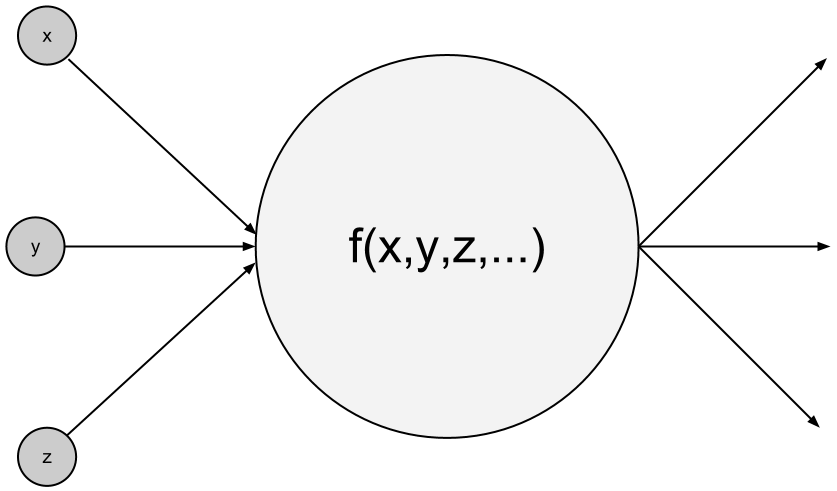
\includegraphics[scale=0.5]{images/neuron.png} \\
    Single neuron with inputs $x$, $y$, $z$ and activation function $f$
\end{center}

This neuron takes a bunch of input values from other neurons, or from the
"environment", somehow processes that data (via an activation function $f$), and
then sends it output to any neurons that it's connected to. We can then layer
these neurons, forming a neural network:

\begin{center}
    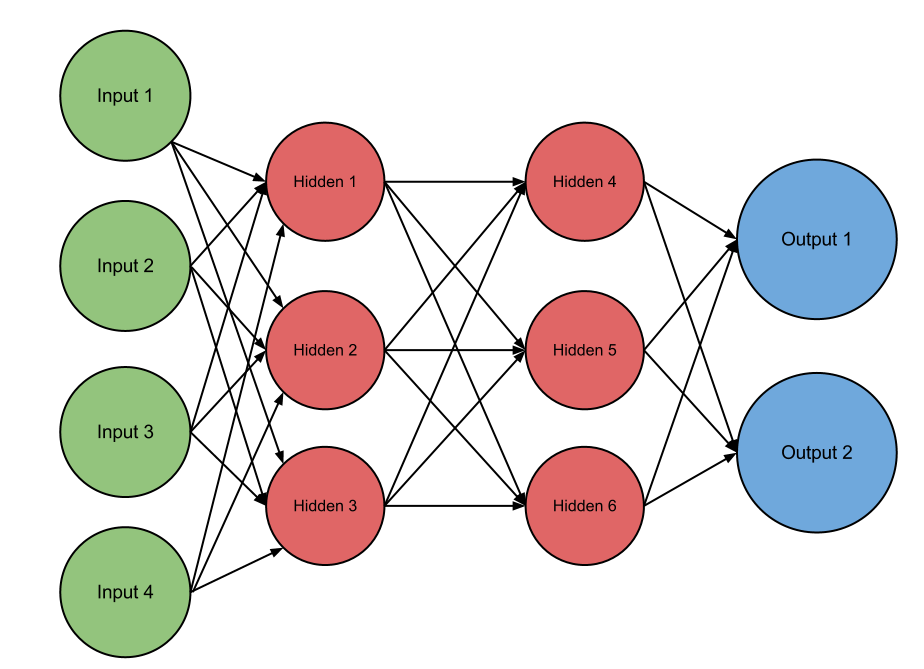
\includegraphics[scale=0.5]{images/neural-network.png} \\
    Neural network with four inputs, two hidden layers (three neurons each), and two outputs
\end{center}

In addition to these input values, each link in the neural network (represented
above by arrows) has an associated weight parameter \(w_i\). When we are
calculating our values, we scale each input by its respective weight. For
instance, in order to calculate the value of the first hidden unit with
activation function $f$, we would compute
\[h_1 = f(w_{1,1}\cdot i_1, w_{2, 1}\cdot i_2, w_{3,1}\cdot i_3, w_{4,1}\cdot i_4)\]
The value \(w_{i, j}\) is the scaling factor for the $i$th input going to the
$j$th hidden unit.

(We can quickly check that this rather complicated model is sufficient for
modeling a linear model: if we allow the activation function to simply be a sum
of the terms, this becomes a multi-variable linear model. This is a silly use
of neural networks, though.)

\subsection*{Activation Functions}

The choice of activation functions is incredibly important when designing a neural network, and
there are a multitude of choices. One common function is just the Heaviside function - if the sum of
the inputs is greater than some threshold T, output one, otherwise, output zero: 
\[U_T(x_1,x_2,\ldots) = \left\{ \begin{array}{lr} 1 & \text{if } \sum x_i > T\\ 0 & \text{otherwise} \end{array} \right. \] 
This corresponds to the biological theory that a real neuron cell either fires (via a voltage
spike) or doesn't. One problem with this activation function - for our purposes - is that since
it is non-differentiable, we cannot use it with gradient descent. Thus, another common
activation function is the logistic function: 
\[f(x_1, x_2, \ldots) = \frac{1}{1 + e^{-x_1-x_2-\ldots}}\]

\begin{center}
    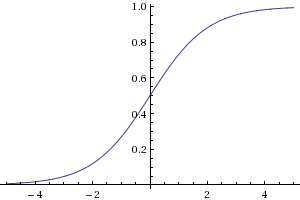
\includegraphics[scale=0.5]{images/logistic.png} \\
    Graph of the logistic function
\end{center}

The logistic function is nice because it is very similar to the step function described above, but
is differentiable, unlike the step function. Thus, the neural networks we'll be talking about will
use the logistic activation function.

\subsection*{Prediction and Learning}

When we are using a neural network, we need to choose the structure (number of neurons in each
layer, number of layers, etc) and then we need to teach the neural network in order to choose the
weight parameters. As described above, to calculate our answer, we simply feed the input layer
values into the activation functions (with the appropriate weights) in order to calculate the values
of the first hidden layer. Then, we feed those values (with appropriate weights, different from the
previous step) into the activation functions in order to calculate the values of the second hidden
layer. We repeat this process until we have the activation values for the output layer. Because of
this process, these networks are called feed-forward neural networks. (In other types, there can be
cycles in the neuron connections and other quirks, which make this sort of forward propagation
algorithm impossible.)

Sadly, prediction is the easy part. The hard part is teaching the neural network the right values
for the weights. We start out by giving the neural network completely random weights. Then, we
iteratively apply gradient descent to teach the neural network the right values for the parameters.
However, for gradient descent, we need to be able to calculate the gradient for any set of
parameters!

To find the gradient, we use a backpropagation algorithm. The backpropagation algorithm is almost
the exact opposite of the feed-forward propagation. We start out by finding the error, or the
difference between the neural network output and the expected output:

\begin{center}
    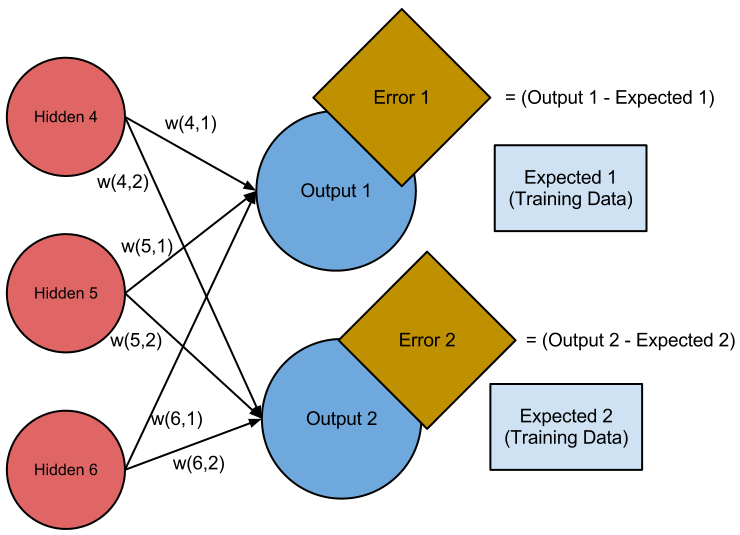
\includegraphics[scale=0.5]{images/backprop-1.png}\\
    First step of backpropagation: error calculation
\end{center}

We would like to minimize this error, in some form. (We can minimize the squared residuals, like we
do when learning a least-squares linear model.) Just from this calculation, we can learn the
parameters we see on screen. The cost of the errors we've already calculated would be: 
\[J_1(h_4, h_5, h_6) = (E_1 - f(w(4,1)h_4, w(5,1)h_5, w(6,1)h_6)^2.\]
where $f$ is the logistic function and $E$ is the expected results (the training data). Since the
logistic function is differentiable, we can take the gradient of this cost (derivative with respect
to $w(4,1)$, $w(5,1)$, and $w(6,1)$) and minimize it with gradient descent.

If we computed the cost and gradient for every unit in the network, we'd be done, as we would've
learned all our parameters. However, we can't - because we only know the expected results for the
output layer. We have no idea what the values in the hidden layer "should" be, so we can't calculate
a cost function. This is where the backpropagation occurs. Just like we propagated values forward,
we now propagate error backwards, using the same exact weights. Thus, if $w(6,2)$ is big, and thus
contributed a lot to the error of output unit 2, we will assign to it a larger value when
backpropagating:

\begin{center}
    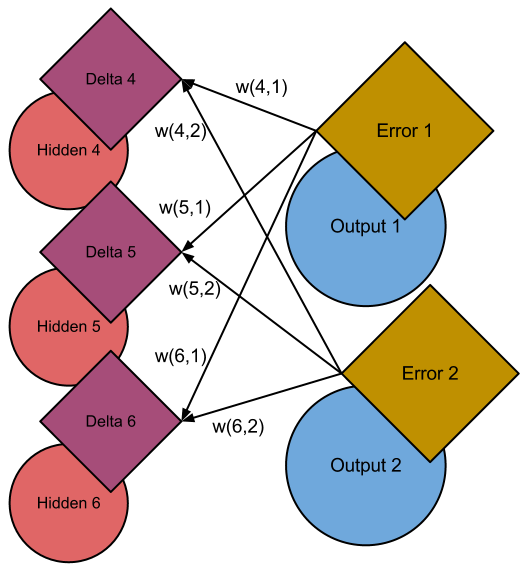
\includegraphics[scale=0.5]{images/backprop-2.png} \\
    Backpropagation to the penultimate layer
\end{center}

We can now repeat this backward propagation until we have deltas for all our units, save, of course,
for the input layer. Since we have deltas for each unit, and our activation function is
differentiable, we can now compute the gradient of our entire neural network. The gradient of the
entire neural network (with respect to the parameters of the network) will then let us apply
gradient descent, and learn the entire set of neural network weights!

\begin{center}
    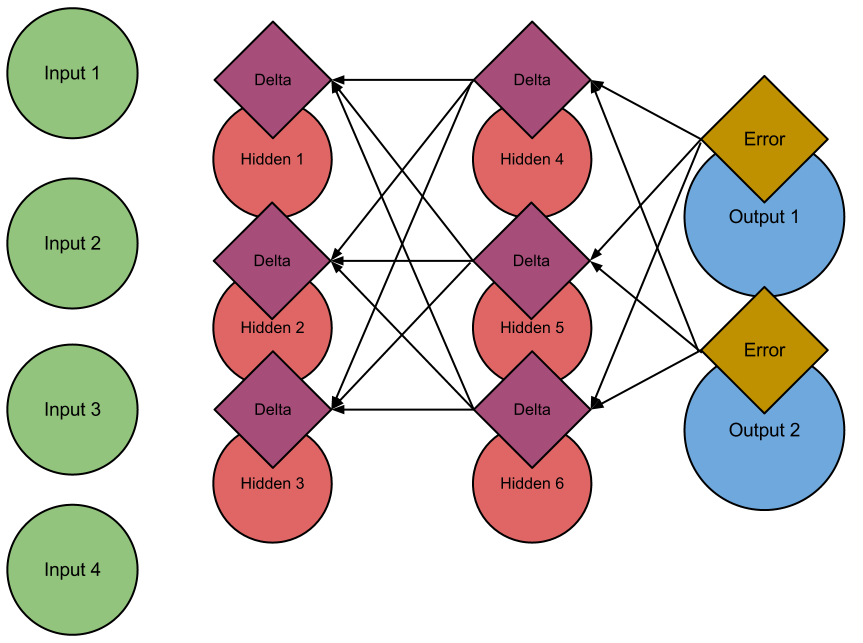
\includegraphics[scale=0.5]{images/backprop-3.png} \\
    Complete backpropagation of error through the network
\end{center}

\subsection*{Applications of Neural Networks}

And now, you hypothetically have the knowledge to go ahead and use neural networks for your own
applications. It's not immediately obvious, however, how to structure a neural networks and what to
use as inputs and outputs. One common application of neural networks is text recognition.

There are plenty of freely available datasets, but a particularly nice and simple one is the
database of USPS handwritten digits. You can access it in Matlab-ready form here. (Thanks to Sam
Roweis at NYU for compiling that awesome website!) It consists of 11,000 20x20 pixel images, each of
which is a single handwritten digit, zero through nine.

\begin{center}
    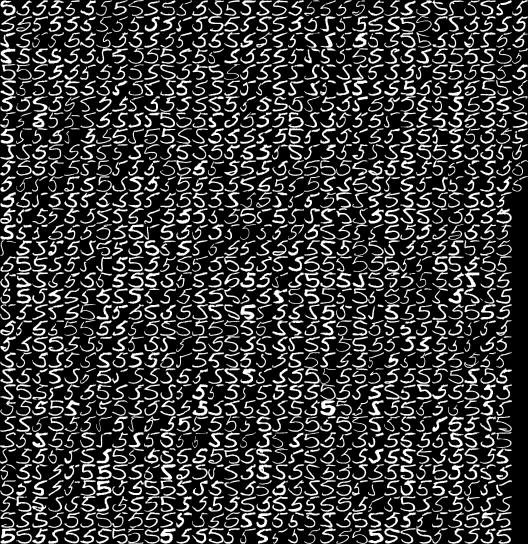
\includegraphics[scale=0.5]{images/usps.jpg} \\
    Sample USPS data for the digit '5'
\end{center}

In order to classify the digits with a neural network, we can create a network with 400 input units
(one per pixel),  one hidden layer with 25 units, and one output layer with 10 units. Each pixel
corresponds to one of the input units, and each output unit corresponds to a digit (0 through 9). If
the image is of a "2", then all but the 3rd (off by one due to the zero) output unit should be a
one, and all the other output units should be a zero. With this in mind, we can train our neural
network on this dataset, since we have the input (images) and the outputs (one for the digit that
the image is of, zero for the others).

If you'd like to take a look at some Matlab code that implements this, take a look at \href{https://github.com/gibiansky/experiments/tree/master/neural-network}{this code}. It
achieves more than 90\% accuracy on USPS data classification. I've tried to keep it clean and
commented!

\textbf{Note:} Using neural networks in production can actually be quite tricky. There are a bunch of little
details that I haven't discussed at all, such as regularization (to prevent overfitting your data),
adjusting the learning rate appropriately, checking whether the model is overfitting or underfitting
the data, etc. If you like this sort of stuff, take an online class on machine learning or neural
networks!
\end{document}
